\documentclass[output=paper]{langscibook} 
\ChapterDOI{10.5281/zenodo.5578834}

\author{Laura McPherson\affiliation{Dartmouth College} and Lucas James\affiliation{Dartmouth College}}
\title{Artistic adaptation of Seenku tone: Musical surrogates vs. vocal music}  
\abstract{The tonal nature of many African languages has long raised questions about musical expression and the relationship between language and music. The two main areas of inquiry have been the relationship between tone and melody in vocal music (tonal textsetting) and the role of tone in musical surrogate languages (e.g. talking drums). However, the degree of similarity between these two genres in terms of tonal adaptation has remained an open question. In this paper, we present a case study comparing the role of tone in two musical traditions from the Sambla ethnic group of Burkina Faso: vocal music and a balafon (xylophone) surrogate language. We show that the two have different systems of tone-note correspondence and level of phonological encoding, indicating that musical adaptation of tone is not monolithic. We suggest that these different systems of tonal adaptation may stem from functional, structural, and cultural differences between the two musical genres.}

\begin{document}
\SetupAffiliations{mark style=none}
\maketitle


\section{Introduction}

There has been nearly a century of scholarly interest in the role of linguistic tone in African music, which can be divided into two areas of study: vocal music and musical surrogate languages (e.g. \citealt{Stern1957,SebeokUmiker-Sebeok1976}). In the study of vocal music, the question is one of tonal textsetting, or tone-tune association: To what extent does linguistic tone constrain the musical melody? The literature spans a diverse range of African languages, including Bantu and Bantoid languages like Xhosa \citep{Starke1930},
Zulu \citep{Rycroft1959,Rycroft1979},
Shona \citep{Schellenberg2009}, and
Fe'Fe' Bamileke \citep{Proto2016};
Chadic languages like Hausa \citep{Richards1972,Leben1983},
as well as other languages of West Africa such as
Ewe (Kwa; \citealt{Jones1959,Hornbostel1928}) and
Tommo So (Dogon;  \citealt{McPhersonRyan2018}).
The results are equally diverse, with some languages like Zulu showing very strict tone-tune matching (92\% parallel movement between tone and tune) and others like Shona showing only a very small influence exerted by tone (just 53\% parallel movement).

The study of musical surrogate languages looks at the way in which a language's phonological material is transposed onto the notes and rhythms of musical instruments to transmit messages. The best known musical surrogate systems are known colloquially as ``talking drums'', a term applied equally to tension drums (e.g. Yorùbá, \citealt{Beier1954}),
slit log drums (e.g. Lokele, \citealt{Carrington1949}), and sets of tuned drums (e.g. Ewe, \citealt{LockeAgbeli1981}). However, musical surrogate languages are found on a variety of instruments, including trumpets (Akan, \citealt{Kaminski2008}), flutes (Sambla, \citealt{McPherson2019a}), string instruments (Benchnon, \citealt{Wedekind1983}), and xylophones (Senoufo, \citealt{ZempSoro2010}).

While each of these areas are interesting in their own right, consideration of just a single tradition on its own makes it difficult to determine similarities and differences in tonal adaptation between both different modalities for a single language (i.e. vocal music vs. surrogate languages) as well as between languages for a single modality (i.e. musical surrogate languages across languages). It thus remains an open question whether there are such things as universals in the artistic adaption of tone. In this paper, we present a case study that aims to address the first generalization by comparing tonal adaptation in Seenku (Mande, Burkina Faso) vocal music and balafon surrogate speech, drawing on data from both primary fieldwork and archival recordings.\footnote{Audio of all examples cited in this paper can be found at \url{https://zenodo.org/record/5219011}.} We compare our results to other findings in the literature with the aim of sketching out some preliminary thoughts on the second generalization, i.e. differences across languages for a particular modality. In the end, we will show that tonal adaptation appears to be sensitive to a number of factors, including modality, instrumental constraints, and communicative function. 

This paper is structured as follows: In \S\ref{sec-Sambla}, we provide a background of the Sambla people, music, and language (Seenku). In \S\ref{sec-balafon}, we turn to the first form of tonal adaptation, balafon surrogate speech; \S\ref{sec-vocal} extends the discussion to vocal music and tonal textsetting. In \S\ref{sec-surrogate-vocal}, we loop back to the balafon to consider ``surrogate textsetting'', before concluding with a discussion of the results in \S\ref{sec-discussion}. 


\section{The Sambla}\label{sec-Sambla}

\subsection{People and language}

The Sambla are a Mande group of people living in southwestern Burkina Faso. The term ``Sambla'' is an exonym (variant spelling: Sembla), often used to refer to both the language and the people. The endonym for the ethnicity is [sɛ̰́ɛ̰]\footnote{We mark nasality in Seenku with a tilde beneath the vowel to avoid diacritic stacking with tone. Tone is marked once per syllable, with the following conventions: super-high (S) = a̋, high (H) = á, low (L) = à, and extra-low (X) = ȁ. In addition, we use the following contour tone diacritics: LS = ǎ, HX = â, SX = ä; all others, found primarily on long vowels, are written as a sequence of two diacritics, e.g. HS = áa̋.}, with the language known as [sɛ̰́ɛ̰-kû], or Seenku. In this paper, we will refer to the people and culture as Sambla and the language as Seenku. 

Seenku [ISO 639-3: sos] is a member of the Samogo group and is spoken by about 15,000 people \citep{McPherson2020}. It has an unusually rich tone system, with four contrastive levels we refer to as super-high (S), high (H), low (L), and extra-low (X); a four-way minimal set for the level tones is shown in (\ref{minimal}):

\begin{exe}
  \ex\label{minimal} \begin{tabular}[t]{ll}
  si̋ &  `tree species' \\
sí  &  `reciprocal (bound pronoun)' \\
sì &  `first son (birth order name)' \\
sȉ &  `water jar'   \\
  \end{tabular}
\end{exe}




The primary acoustic correlate of tone is f0 \citep{McPherson2019b}.

In addition to the level tones, the language boasts multiple contour tones, including two-tone contours like HX \textit{gɔ̂ɔ} `wood', LS \textit{gɔ̌ɔ} `dry', or HX \textit{ŋáa̋} `yawn', as well as three-tone contours like XHX \textit{gɔ̏ɔ̂n} `sorrel', LSX \textit{kàä} `gone (perfect)', and HXS \textit{dôőn} `child (past subject)', among others. In contrast to the complex tone system, word structure is relatively simple, with the vast majority of Seenku vocabulary being either monosyllabic or ``sesquisyllabic'' \citep{Matisoff1990,Pittayaporn2015}, i.e. words like \textit{məni̋} `woman' or \textit{səgȁ} `sheep' consisting of a short half syllable followed by a full syllable. The only coda consonant is a nasal \citep{McPherson2020}, and the syllable nucleus can contain either a monophthong or a diphthong, either of which may be short or long (e.g. \textit{kȕa} `cultivate (tr.)' vs. \textit{kȕaa} `cultivate (intr.)').

\subsection{Sambla music}

The oldest Sambla instruments include a tension drum known as \textit{dənṵ̏}, a barrel drum in different sizes known as \textit{də̏nḭ̋}, a whistle known as \textit{sɔ̂}, a wooden traverse flute known as \textit{pîɔn}, and a horn known as \textit{gbɛ̂n}. Of these traditional instruments, only the tension drum and the whistle are seen in frequent use today. This is due in large part to the arrival in Sambla country of the balafon, a resonator xylophone, near the end of the 19th century \citep{Strand2009}. Adapted from the neighboring Tusia ethnicity, the balafon has become the most important Sambla instrument and a strong marker of cultural identity.

Most Sambla music is based on vocal music, including praise songs, work songs, and lullabies, which also predate the arrival of the balafon. Unfortunately, much of the vocal repertoire is being forgotten. 


\section{Talking balafons}\label{sec-balafon}

The Sambla balafon belongs to a family of resonator xylophones found throughout West Africa. The resonance comes from tuned gourds that hang beneath each wooden key, amplifying the sound. The traditional Sambla balafon has 23 keys and is tuned to a pentatonic scale. \tabref{tab:mcpherson:Sambla} provides the names of the notes in Seenku, along with the closest corresponding Western scale degree. There are a few interesting things to note here: First, the tonic (1) and its octave (8) have different names. Second, the third and fifth are named in reference to these notes, but the references are {\sc spatial}; the third is ``below'' the tonic, since higher notes have smaller gourds and are hence closer to the ground, with the opposite relation holding between the sixth and the octave of the tonic. In the transcriptions that follow, we will refer to both the abbreviated Seenku name as well as the Western scale degree to maximize clarity. 
 
\begin{table}
  \caption{Sambla pentatonic scale\label{tab:mcpherson:Sambla}}
  \begin{tabular}{llll} 
    \lsptoprule
Western & Sambla & Abbrev. & Translation \\ 
 \midrule
    1 & bâ̰a̰-ɲȁ & B &  lit. `balafon mother' \\
    b3 & jîo-bȁ̰a̰-dȅn & J & lit. `fetish balafon key' \\
    3 & bâ̰a̰-ɲȁ-gṵ̏-nɔ̰̏n & Bg & lit. `the one under balafon mother' \\
    5 & tərɔ́n-tərɔ́n & T &  (no translation) \\
    6 & sərà-kùa-kɔ̀-nɔ̰̀n & Sk &  lit. `the one above \textit{sərȁ-kȕa} \\
    8 & sərȁ-kȕa & S &  (no translation) \\ 
      \lspbottomrule
  \end{tabular}
\end{table}

The balafon is found at all major village events, including marriages, funerals, large farming work parties, spiritual ceremonies, and other holidays. A single instrument is played by three players at once, with a simple middle part, a more complex bass line, and the most advanced player acting as the soloist on the treble keys. 

The Sambla balafon is notable in that it is not simply a musical instrument: It is a mode of communication, with a complex speech surrogate system. The soloist is responsible for the surrogate speech, and it is his\footnote{Traditionally, the balafon and other instruments are restricted to men, with women largely dominating vocal music.} job to communicate with dancers, spectators, and the spiritual world through the words of the musical language. It is this system that forms the focus of our discussion in this paper. For more in-depth discussion of cultural and musicological aspects of the Sambla balafon, see \citet{Strand2009}.

Communication on the balafon is achieved by encoding aspects of Seenku phonological structure, namely tone and word shape; segmental contrasts play no role at all. \citet{McPherson2019a} describes the grammar of the surrogate system in depth, drawing on a corpus of primary data gathered with members of the Diabaté clan on balafonists from Torosso, Burkina Faso. In this paper, we will focus on  the rules of tonal adaptation in order to form a basis of comparison with tonal adaptation in vocal music.

Broadly speaking, Seenku tone gets encoded in the notes of the balafon. To illustrate, we can consider the following frame sentence played on the balafon:

\ea 
\gll \underline{\hspace{1cm}} nǎ səmâ \\
\underline{\hspace{1cm}} {\sc prosp} dance \\
\glt `\underline{\hspace{1cm}} will dance.' 
\z 

We can substitute in subject pronouns with different tones, like \textit{mi̋} `1pl', \textit{mó} `1sg', or \textit{mɔ̰̏} `3sg generic' (similar to English `one' or French \textit{on}). The balafon transcription in Figure~\ref{will-dance} is organized as follows: Notes are shown down the lefthand side, both with their abbreviated Seenku names and with their corresponding Western scale degrees. The words are laid out along the bottom, with the shaded cells indicating a note strike. In this example, the horizontal stripes correspond to S-toned \textit{mi̋}, the crosshatching corresponds to H-toned \textit{mó}, and the vertical stripes correspond to X-toned \textit{mɔ̰̏} (\figref{will-dance}).

\begin{figure}
  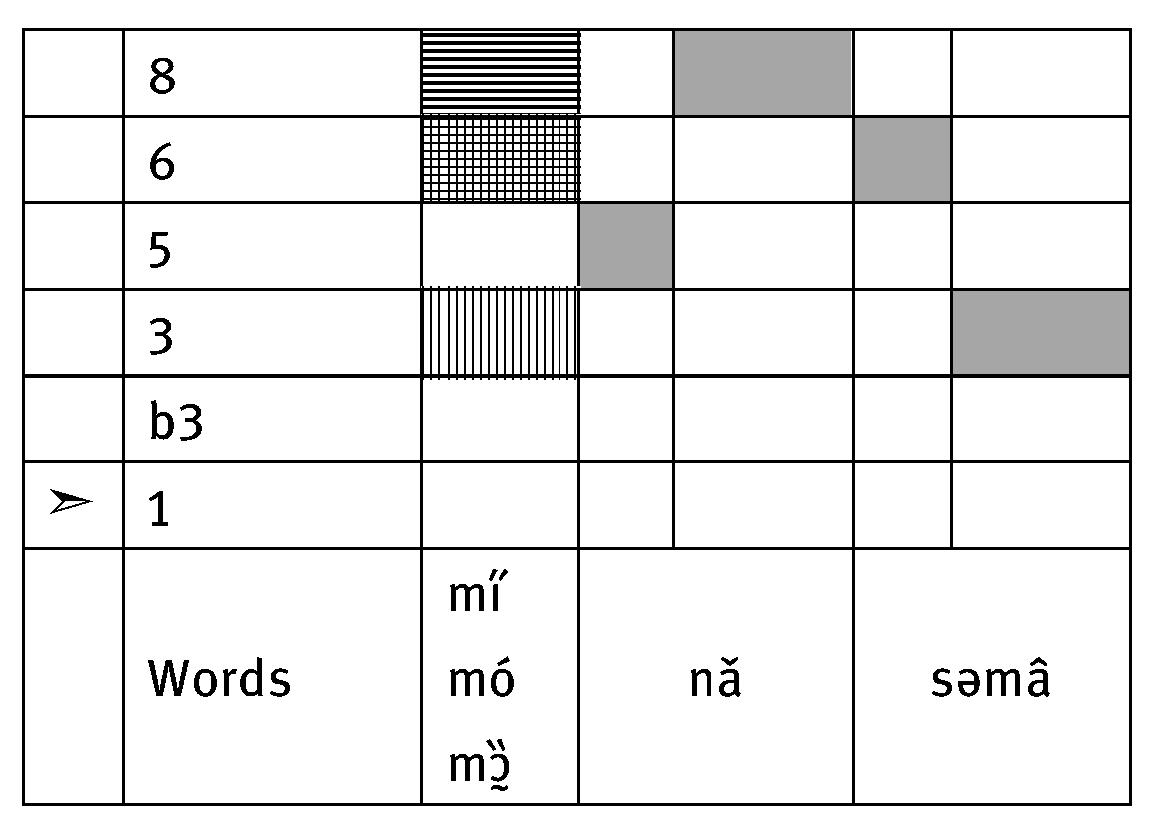
\includegraphics[scale=.4]{figures/mi-mo-ex.eps}
  \caption{Balafon transcription of  `\underline{\hspace{1cm}} will dance'}\label{will-dance}  
\end{figure}

Thus, as this example shows, surrogate tone is relative, with higher tones corresponding to higher notes. 

However, it is not the case that any particular key (e.g. the \textit{tərɔ́n-tərɔ́n}, or 5th) uniformly encodes a particular tone; rather, speech surrogate tone, like spoken tone, is relative and dependent upon the {\sc musical mode} of the song, i.e. which note acts as the melodic center for that particular song. The most common musical mode, and the one used as a default for surrogate speech if the musician has no other song in mind, is centered around the \textit{bâ̰a̰-ɲȁ/sərȁ-kȕa}, hence its designation as ``1''. The bias towards this mode is noticeable when we consider the distribution of tones to notes across our data corpus (consisting of around 800 words on the balafon), shown in \tabref{tab:mcpherson:tonenote}. 

\begin{table}
 \caption{Tone-note correspondence in the balafon surrogate corpus\label{tab:mcpherson:tonenote}} 
\begin{tabular}{lrrrrrr} 
\lsptoprule
   & {1} & {b3} & {3} & {5} & {6} & {8} \\ \midrule
   S & 0 & 1 & 8 & 22 & 38 & \textbf{158} \\ 
   H & 4 & 0 & 72& 85 & \textbf{154} & 28 \\ 
   L & 2 & 1 & 9 & \textbf{73} & 15 & 7 \\ 
   X & \textbf{101} & 2 & \textbf{93} & 57 & 14 & 15 \\
\lspbottomrule
\end{tabular} 
\end{table}

The numbers in boldface represent the most common note for that particular tone category; for instance, S is most commonly played on the \textit{sərȁ-kȕa} (8) in our corpus, H on the \textit{sərà-kùa-kɔ̀-nɔ̰̀n} (6), etc. The lowest tone, X, is split almost evenly between the \textit{bâ̰a̰-ɲȁ-gṵ̏-nɔ̰̏n} (3) and the \textit{bâ̰a̰-ɲȁ} (1). These represent the most common setting of tones to notes in the mode centered on the \textit{bâ̰a̰-ɲȁ}, but in other modes, we tend to see S tied to the center of the mode (in the higher octave), with the other tones cascading down from there. To give an example, in the \textit{tərɔ́n-tərɔ́n} mode, S would be encoded on this note, H below that on the 3rd, etc. 

Looking at \tabref{tab:mcpherson:tonenote}, the astute reader may notice a conspicuous absence of tone encoding on the \textit{jîo-bȁ̰a̰-dȅn} (b3). Recall that the translation of this key name is the ``fetish balafon key'', and as such, it tends to be reserved for spiritual uses and is only seldom active in surrogate speech. 

Contour tones are encoded on the balafon by playing each of the component tones. For two-tone contours, these two notes are played as a flam, i.e. the two notes in rapid succession. The example in (\ref{thirst}) contains two contour tones, an HL contour tone (indicated with a sequence of acute and grave accent to distinguish it from the more common HX 〈â〉) and an LS contour tone. In both cases, the component tones are clearly played on the correponding balafon notes:

\ea\label{thirst} 
\ea
 \gll {jʊ́ ̀-mərḭ̀} nǎ mó bȍ təgòn-təgòn \\
water-drink.{\sc antip.nom} {\sc prosp} {\sc 1sg.emph} kill.{\sc irr} {\sc red-}completely \\
\glt `I am dying of thirst.' (Lit. thirst will kill me completely) \\
\ex \attop{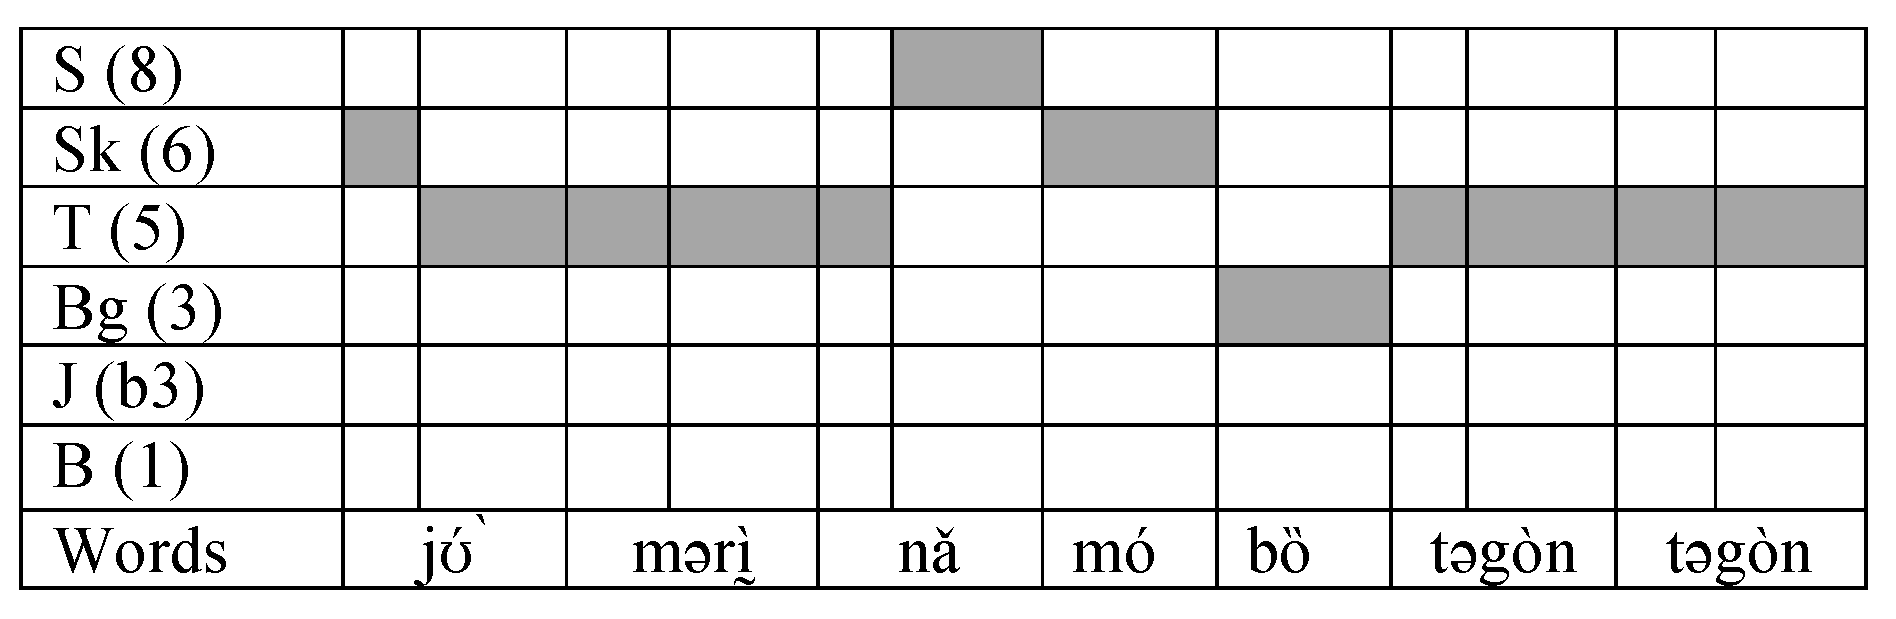
\includegraphics[scale=.3]{figures/thirst2.eps}}
\z
\z

The relative width of the columns reflects the amount of time between strikes; for the HL contour tone in the first word, the note on \textit{sərà-kùa-kɔ̀-nɔ̰̀n} (6) encoding the H tone is shorter than the following L tone on \textit{tərɔ́n-tərɔ́n} (5). 

While both level and contour tones are encoded on the balafon, we must ask what level of tone is being represented. Like phonology more generally, tone is nuanced and multilayered, including (at least) lexical/underlying tone, grammatical tone, postlexical tone, and phonetic tone. One of the most interesting findings of the balafon surrogate language is that only the first two categories are encoded, i.e. lexical and grammatical tone. More surface-level effects, including the output of postlexical tone rules and details of phonetic implementation, are not encoded. 

Consider the following example:

\ea\label{buy-goats}
\gll mó nǎ bi̋ sa̰̋   \\
{\sc 1sg.emph} {\sc prosp} goat.{\sc pl} buy.{\sc irr} \\
\glt `I will buy goats.' \\
\z

The tonal forms shown in (\ref{buy-goats}) include both lexical tone and grammatical tone, but no postlexical effects, which we will discuss shortly. The first two words, \textit{mó} and \textit{nǎ}, are both shown with only lexical tone. The object noun \textit{bi̋} `goats' is underlyingly H-toned /bí/, but it raises to superhigh tone due to a featural affix [+high] marking the plural \citep{McPherson2017morphology,McPherson2017acal}. This S tone then spreads onto the lexically X-toned verb /sȁ̰/ `buy' through the process of argument-head tone sandhi, a morphosyntactically-constrained sandhi process argued in \citet{McPherson2019c} to be a case of allomorph selection.

When the form in (\ref{buy-goats}) is pronounced, it is realized as [mó nà !bi̋ sa̰̋], with two postlexical tone processes. The first is tonal absorption   \citep{HymanSchuh1974}, a kind of rising tone simplification in which an LS-S sequence is simplified to L-S. After this L tone, the S of \textit{bi̋} undergoes downstep, leaving it pronounced at the same level as the preceding H tone.

The transcription in Figure~\ref{buy-goats-balafon} shows how this phrase is realized in the balafon surrogate language.


\begin{figure}
  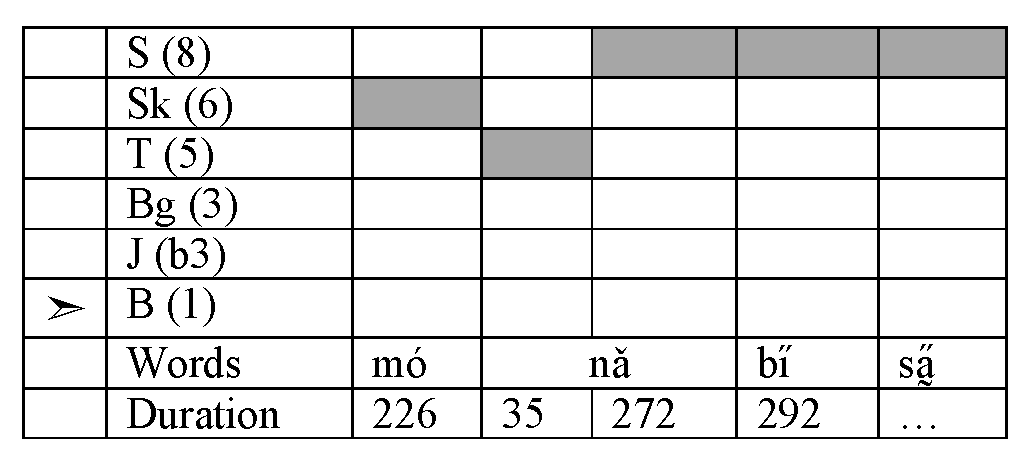
\includegraphics[scale=.5]{figures/i-will-buy-goats.eps}
  \caption{Balafon transcription of 'I will buy goats'}\label{buy-goats-balafon} 
\end{figure}


As this example clearly shows, the auxiliary \textit{nǎ} retains its LS rising tone on the balafon. The object noun \textit{bi̋} is played on the same note as the end of the rising tone, showing that it has raised to S, which likewise spreads onto the verb. In other words, grammatical tone processes (both morphological tone and argument-head tone sandhi) are both encoded in balafon surrogate speech while postlexical tone (rising tone simplification and downstep) is not. 

This result is surprising if we expect tonal adaptation in surrogate speech to resemble tonal textsetting -- many studies of tonal textsetting (e.g.
Hausa, \citealt{Leben1983};
Yorùbá, \citealt{Villepastour2014};
Kpelle, \citealt{KonoshenkoKuznetsova2015};
Tlahuapa Tù'un Sàví, \citealt{Sleeper2018})
demonstrate that what is encoded is a surface level of tone rather than something closer to the underlying form. We are thus left with the following hypotheses:

\begin{enumerate}
  \item Seenku tone is musically adapted differently from the common pattern found in other languages like those cited above, perhaps due to its level of complexity.
  \item Surrogate languages adapt tone differently from sung music, perhaps because the message is reduced to simply tone (and rhythm) thus increasing the functional load of tone or because the purpose of surrogate speech is communication rather than artistic expression per se.
\end{enumerate}

To probe these hypotheses, we turn in the next section to a preliminary study of tonal textsetting in Seenku vocal music. As we will see, the results lend more support to hypothesis 2 than hypothesis 1. 

\section{Vocal music}\label{sec-vocal}

Here we report on the results of a pilot study looking at five Seenku songs. Three of the songs are praise songs, sung by a female griot (musician/historian caste), one is a festival song sung by a woman, and one is a spiritual song sung by a man. The corpus is currently too small to test differences in tone-tune association between genres, but anecdotally, there are no noticeable differences. The three praise songs come from a video recording of a performance in the 1980s. The other two were recorded in 2017 as part of the first author's documentation of Seenku, using a Zoom Q8 video recorder and a Shure SM-93 lavalier recorder. The corpus remains small at the moment due to a combination of available recordings and the time consuming nature of musical transcription, tonal verification, and translation. 

We first transcribed the vocal melodies by hand into musicXML format along with their lyrics. We converted the lyrics to simply their tones, coding tone numerically ranging from 4 (S) to 1 (X). We then ran a python script that reads in the musicXML, with parameters set to identify the Sambla scale degrees and the number of tonal primitives. From this information, the script calculates the degree of correlation between tone and melody. 

If tonal adaptation in vocal music behaved the same as surrogate speech, we might expect to see a distribution of tones and notes comparable to what we saw in \tabref{tab:mcpherson:tonenote}. Instead, we find the results in \tabref{tab:mcpherson:tonenote2}. The octaves are collapsed into a single category here, because phrases in vocal music (unlike those in surrogate speech) are free to span multiple octaves, negating the significance of a higher and lower octave boundary. 

\begin{table}
 \caption{Tone-note correspondence in the vocal music corpus\label{tab:mcpherson:tonenote2}} 
\begin{tabular}{lrrrrr}
\lsptoprule
   & {1/8} & {b3} & {3} & {5} & {6} \\ \midrule
   S & \textbf{35} & 1 & 18 & 16 & 24 \\ 
   H & 64 & 1 & 76 & \textbf{103} & 34  \\ 
   L & 26 & 0 & 15 & \textbf{30} & 7  \\ 
   X & \textbf{70} & 1 & 41 & 46 & 33  \\ \lspbottomrule
\end{tabular}
\end{table}

Rather than a stepwise distribution of each tone appearing one note above the next, we find a much more even distribution across the notes of the scale; however, the avoidance of the \textit{jîo-bȁ̰a̰-dȅn} (b3) is retained.

The study of tonal textsetting tends not to consider absolute correspondences between tones and notes but rather the transitions between two notes and tones. These transitions can be classified by the extent to which the two correspond: Given tones A and B sung on notes X and Y, the transition is parallel if both go the same direction (i.e. rising tone/rising melody, falling tone/falling melody, level tone/level melody); it is contrary or opposing if the transition between A and B goes in the opposite direction as the transition from X to Y (i.e. rising tone/falling melody, falling tone/rising melody); and the transition is oblique if one pair remains level while the other rises or falls (e.g. rising tone/level melody, level tone/falling melody, etc.). See \citet{Schellenberg2012} and \citet{LaddKirby2020} for further discussion.

If we re-examine the results in this light, we find a very strict match between tone and melody in Sambla vocal music. These results are shown in \tabref{tab:mcpherson:Relationship}. In this table, parallel cells are white, oblique cells are in light gray, and contrary cells are in black. As the results show, a remarkable 75.6\% of the corpus is parallel and only 2\% contrary. In terms of the literature on tonal textsetting, Seenku represents a case towards the stricter end of the spectrum. 


\begin{table}[p]
  \caption{Relationship between tonal bigrams and musical bigrams in Seenku vocal music\label{tab:mcpherson:Relationship}}
% %   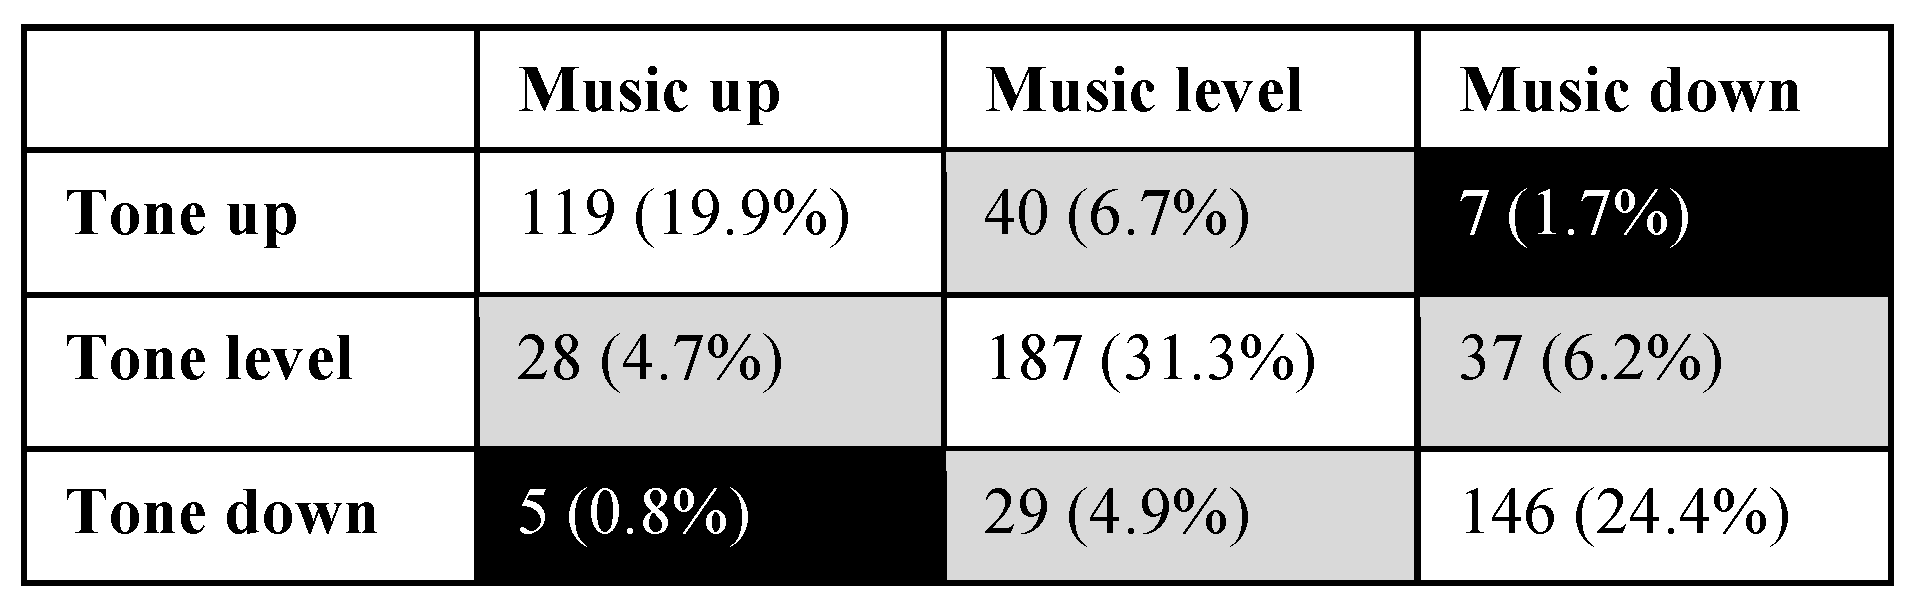
\includegraphics[scale=.33]{figures/Tone-tune-table.eps}
   \begin{tabular}{l *{3}{rr}}
   \lsptoprule
    & \multicolumn{2}{c}{Music up} & \multicolumn{2}{c}{Music level} & \multicolumn{2}{c}{Music down}\\\midrule
    Tone up    & 119 & 19.9\% & \cellcolor{lightgray} 40  & \cellcolor{lightgray} 6.7\%  & \cellcolor{black}\color{white}{7}   & \cellcolor{black}\color{white}{1.7\%}\\
    Tone level & \cellcolor{lightgray} 28  & \cellcolor{lightgray} 4.7\%  & 187 & 31.3\% & \cellcolor{lightgray}37  & \cellcolor{lightgray}6.2\%\\
    Tone down   & \cellcolor{black}\color{white}{5}  & \cellcolor{black}\color{white}{0.8\%}  & \cellcolor{lightgray}29  & \cellcolor{lightgray}4.9\%  & 146 & 24.4\%\\
    \lspbottomrule
   \end{tabular}
\end{table} 


When we look closer, we find that not just the direction of the interval matters for Seenku vocal music, but the size also. First, as shown in Figure~\ref{fig:transitions:size}, contrary mapings are avoided more strongly in larger musical intervals, a result mirrored in other musical traditions such as Tommo So \citep{McPhersonRyan2018}. For instance, if we consider the falling tonal transition in the righthand column, a small number are found on musical intervals that rise by one scale degree (light orange), an even smaller number on musical intervals that rise by two scale degrees (darker orange), and none on musical intervals that rise by three scale degrees.

\begin{figure}[p]
  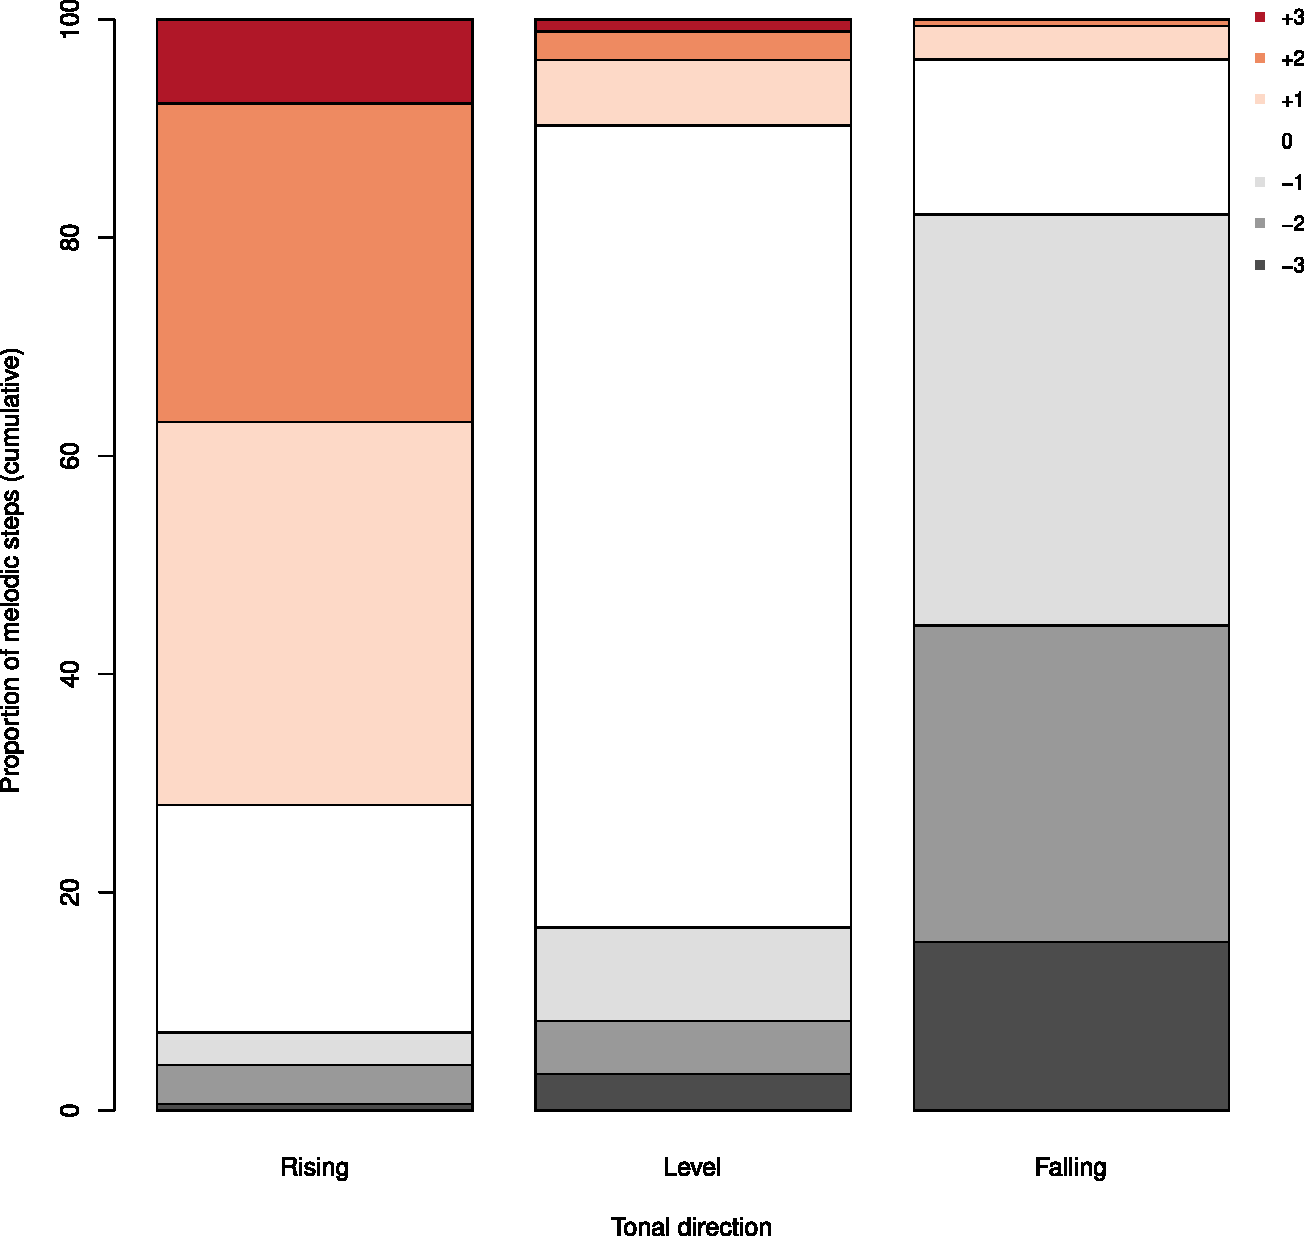
\includegraphics[width=\textwidth]{figures/TonalInterval.pdf}
  \caption{Tonal transitions by interval size\label{fig:transitions:size}}
\end{figure}

In addition to regulating the strictness of match between tone and tune, we also find that musical interval size also correlates closely with tonal interval size, such that larger tonal intervals (e.g. X to S vs. X to H) tend to be set on larger musical intervals. 

\begin{figure}
  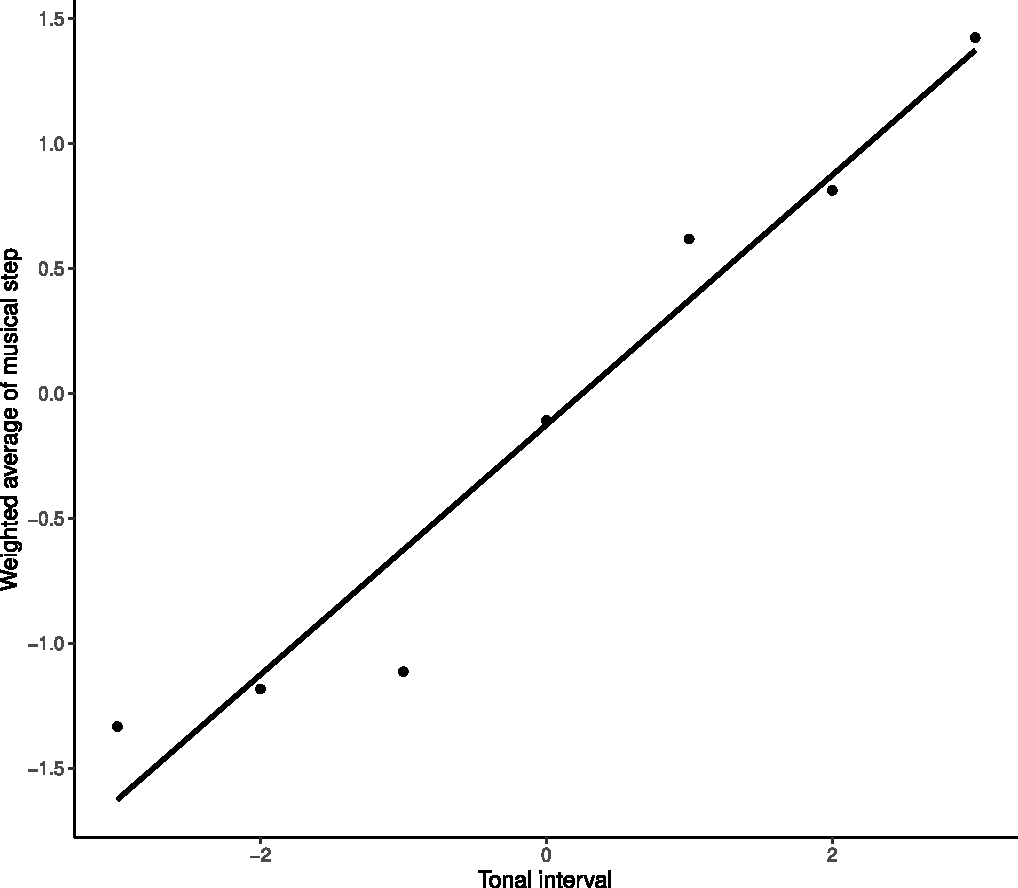
\includegraphics[width=.66\textwidth]{figures/WeightedAverageScatter.pdf}
  \caption{Correlation between tonal transitions and interval size\label{fig:mcpherson:WeightedAverageScatter}}
\end{figure}

As \figref{fig:mcpherson:WeightedAverageScatter} shows, the trend is particularly apparent for rising intervals. 

To summarize what we have seen so far, there are no strong tone-note correspondences in tonal textsetting as there were for balafon surrogate speech (at least within a mode). Instead, we see strict directional textsetting of the sort reported in many other tone languages. The question remains, however: What level of tone does tonal textsetting encode? 

Preliminary results suggest that here too textsetting diverges from surrogate speech in that postlexical tone is encoded. Consider the following line from \textit{The Chief of Bouendé's Song}, along with interlinear glossing:

\ea\label{lyrics1} 
\gll \textit{í} \textit{wó} \textit{nǎ} \textit{wɛ́} \textit{ɲìi} \textit{gȕɔ-fḭ̋ɛ̰-nɛ̋} \textit{kɔ̌ɔ} \textit{je̋n} \textit{ŋɛ́} \\
{\sc log} {\sc emph} {\sc prosp} {\sc foc} be.afraid.{\sc irr} night walk.{\sc nom} in.front {\sc neg} \\
\glt `I will not be afraid to walk at night.'
\z 

When spoken, this line would undergo three postlexical tone processes: (1) The prospective auxiliary \textit{nǎ} would simplify to !S; (2) The nominalized verb \textit{kɔ̌ɔ} would undergo tonal absorption to L before \textit{je̋n} (incidentally only S-toned due to argument-head tone sandhi triggered by the S of \textit{kɔ̌ɔ}); (3)  We would find progressive downdrift across the line, with each S tone following an X or L tone lower than the preceding one. In other words, the surface form would look something like [í wó !na̋ wɛ́ ɲìi gȕɔ-!fḭ̋ɛ̰-nɛ̋ kɔ̀ɔ !je̋n ŋɛ́]. 

Interestingly, unlike on the balafon, all of these postlexical tone processes can be seen in the tonal textsetting. Figure~\ref{fig:songline:bouendechief} shows the musical transcription of the line in (\ref{lyrics1}). 

 \begin{figure}
  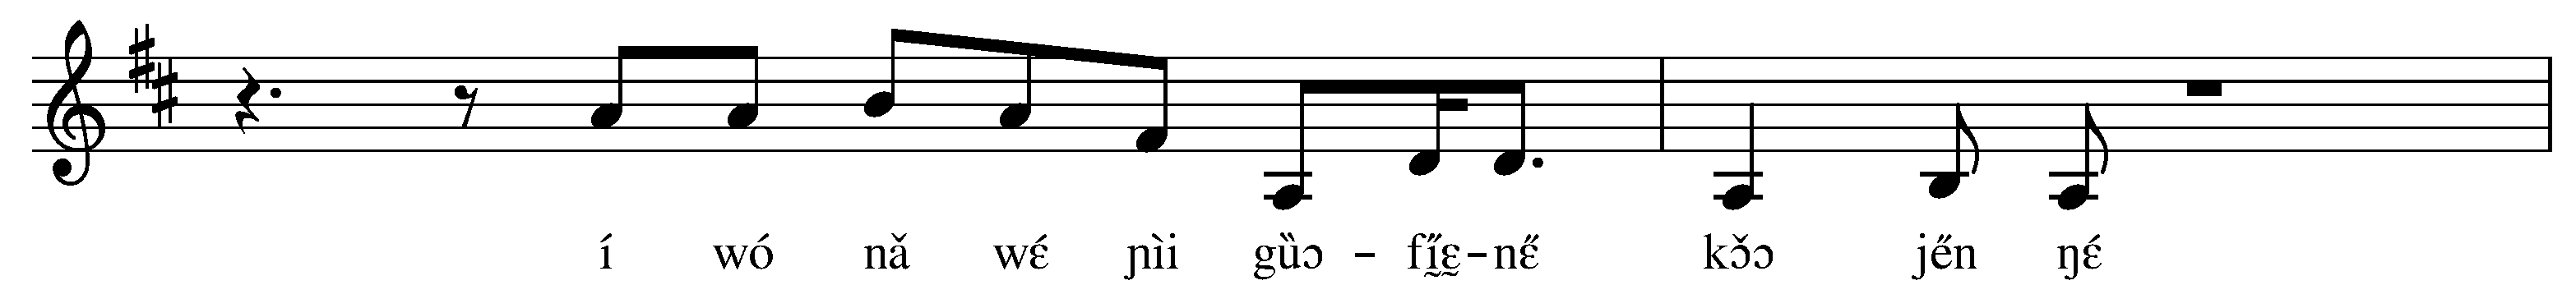
\includegraphics[width=\textwidth]{figures/scared-line.eps}
  \caption{Line from \textit{The Chief of Bouende's Song}\label{fig:songline:bouendechief}}
\end{figure}

First, we find rising tone simplification both to !S and to L reflected in the melody. Both \textit{nǎ} and \textit{kɔ̌ɔ} are sung on a single note (rather than a melisma), with \textit{nǎ} sung on a note higher than the note of the preceding and following H tones and \textit{kɔ̌ɔ} sung on a note lower than both the preceding and following S tones. Further, each subsequent S tone in the line is sung on a note lower than the preceding one, suggesting encoding of downdrift. Of course, it may also be the case that the musical aesthetic prefers falling lines to rising ones, but it is difficult to disentangle even this fact from natural speech prosody. 

To summarize what we have seen in this section, the adaptation of tone in Seenku textsetting differs considerably from what we saw in balafon surrogate speech: First, textsetting is almost entirely relational, requiring the musical and tonal bigrams to match in direction, rather than absolute in tone-to-note correspondence. Second, tone is encoded at a more surface level, including the output of postlexical tone rules such as contour tone simplification and downdrift. 

Before we conclude and discuss these differences between vocal music and instrumental surrogates, we first return to the Sambla balafon one last time in \S\ref{sec-surrogate-vocal} to discuss an intermediate case of tonal adaptation: ``singing balafons''. 

\section{Singing balafons: Surrogate vocal music}\label{sec-surrogate-vocal}

In \S\ref{sec-balafon}, we laid out the principles of encoding of the Sambla talking balafon, a generative speech surrogate system that allows the musician to productively communicate with those around him. In fact, the balafon has two distinct modes of surrogacy, this ``speech mode'' we already covered and a ``sung mode''.  While the speech mode is generative, the sung mode does not appear to be. It appears only during the course of songs, with all three balafonists playing, and consists of much more fluid phrases with highly proverbial meanings. These lines provided quite a puzzle in early stages of analysis, since they often deviated substantially from the apparent rules as defined by the speech mode.

As an example, consider the line in (\ref{blood}): 

\ea\label{blood} 
\gll ȉ kɛ́ mó ń jó wɛ́ ŋəmȁ sḭ̌ nəgȉ nɛ̏ òo \\
{\sc comp} {\sc cop} {\sc 1sg.emph} {\sc 1sg} say.{\sc irr} {\sc foc} blood be cow {\sc loc} {\sc excl} \\
\glt `I said there is blood in a cow.' \\
\z 

Rendered on the balafon, the line comes out as shown in Figure~\ref{blood-balafon}. 

\begin{figure}
  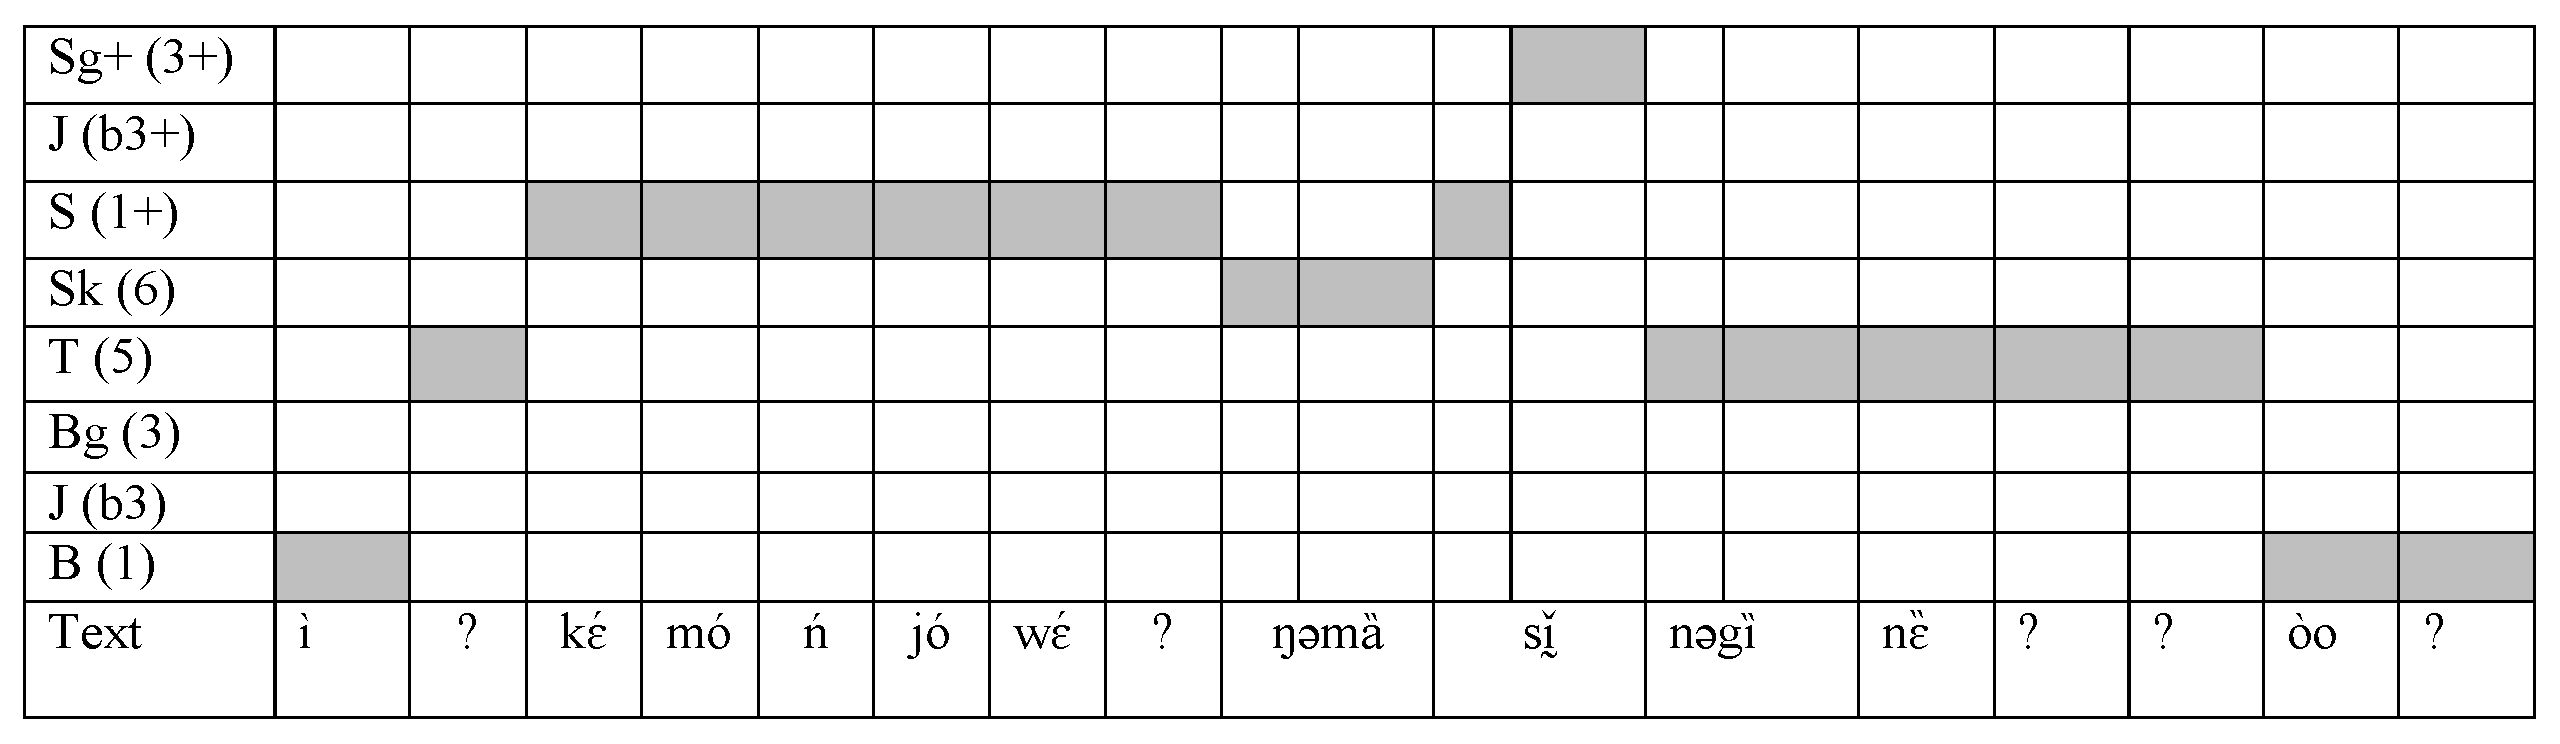
\includegraphics[scale=.4, angle=90]{figures/gbene-gosera-so-balafon.eps}
  \caption{Balafon transcription of `I said there is blood in a cow.'}\label{blood-balafon} 
\end{figure} 

As we can see, there are more notes than expected. In certain places, we can anchor the words to the notes thanks to the rhythm and/or tonal pattern (e.g. \textit{ŋəmȁ sḭ̌} consists of two flams, the first on the same note for the sesquisyllabic X-toned noun and the second on two notes representing the LS contour tone). But in others, such as the long level stretches, it is unclear exactly how the words should map onto the balafon. Further, the relationship between tones and notes is less strict than we would expect if it followed the same rules laid out in \S\ref{sec-balafon}: The initial X tone is considerably lower than that of either \textit{ŋəmȁ} `blood' or \textit{nəgȉ} `cow', which also differ from one another; and the L at the beginning of \textit{sḭ̌} is played on the same note as the level H stretch of \textit{kɛ́ mó ń jó wɛ́}. 

All in all, it is clear we are dealing with a different system of rules in the sung mode than the speech mode. However, as it turns out, we already have the tools for understanding these lines at our disposal as they appear to be a case of ``surrogate singing'' or ``surrogate textsetting''. In other words, the same rules of tonal textsetting and the relationship between tone and sung melody are at play in these ``sung'' lines of the balafon. Looking at the transcription in Figure~\ref{blood-balafon}, we see first that the melody rises from the X tone of \textit{ȉ} to the H tone of \textit{kɛ́} then remains level. It drops going from H to X on \textit{ŋəmȁ} then rises through the rising contour tone of \textit{sḭ̌}, before dropping again to the X of \textit{nəgȉ}. The only deviation is the falling melody moving from the X tones to the L-toned exclamative \textit{òo}. But of course, tonal textsetting is not 100\% strict, and it may also be the case that \textit{òo} in this case is more of a vocable, an artistic flair, than a proper grammatical element with its own fixed tone. 

This explanation makes sense historically, since Sambla oral history states that vocal music predates the balafon, and that when the instrument was introduced, it started playing the songs that were already being sung. In fact, in some performances, we find that the lines of a song are still passed back and forth between a singer and the balafon soloist, allowing us to directly compare the renditions and so the tonal adaptation and answer the question of whether surrogate singing follows exactly the same rules as vocal singing. 

To answer this question, let us return to some lines from the \textit{Chief of Bouendé's Song}, shown in \figref{fig:mcpherson:Bouende}. 

\begin{figure}
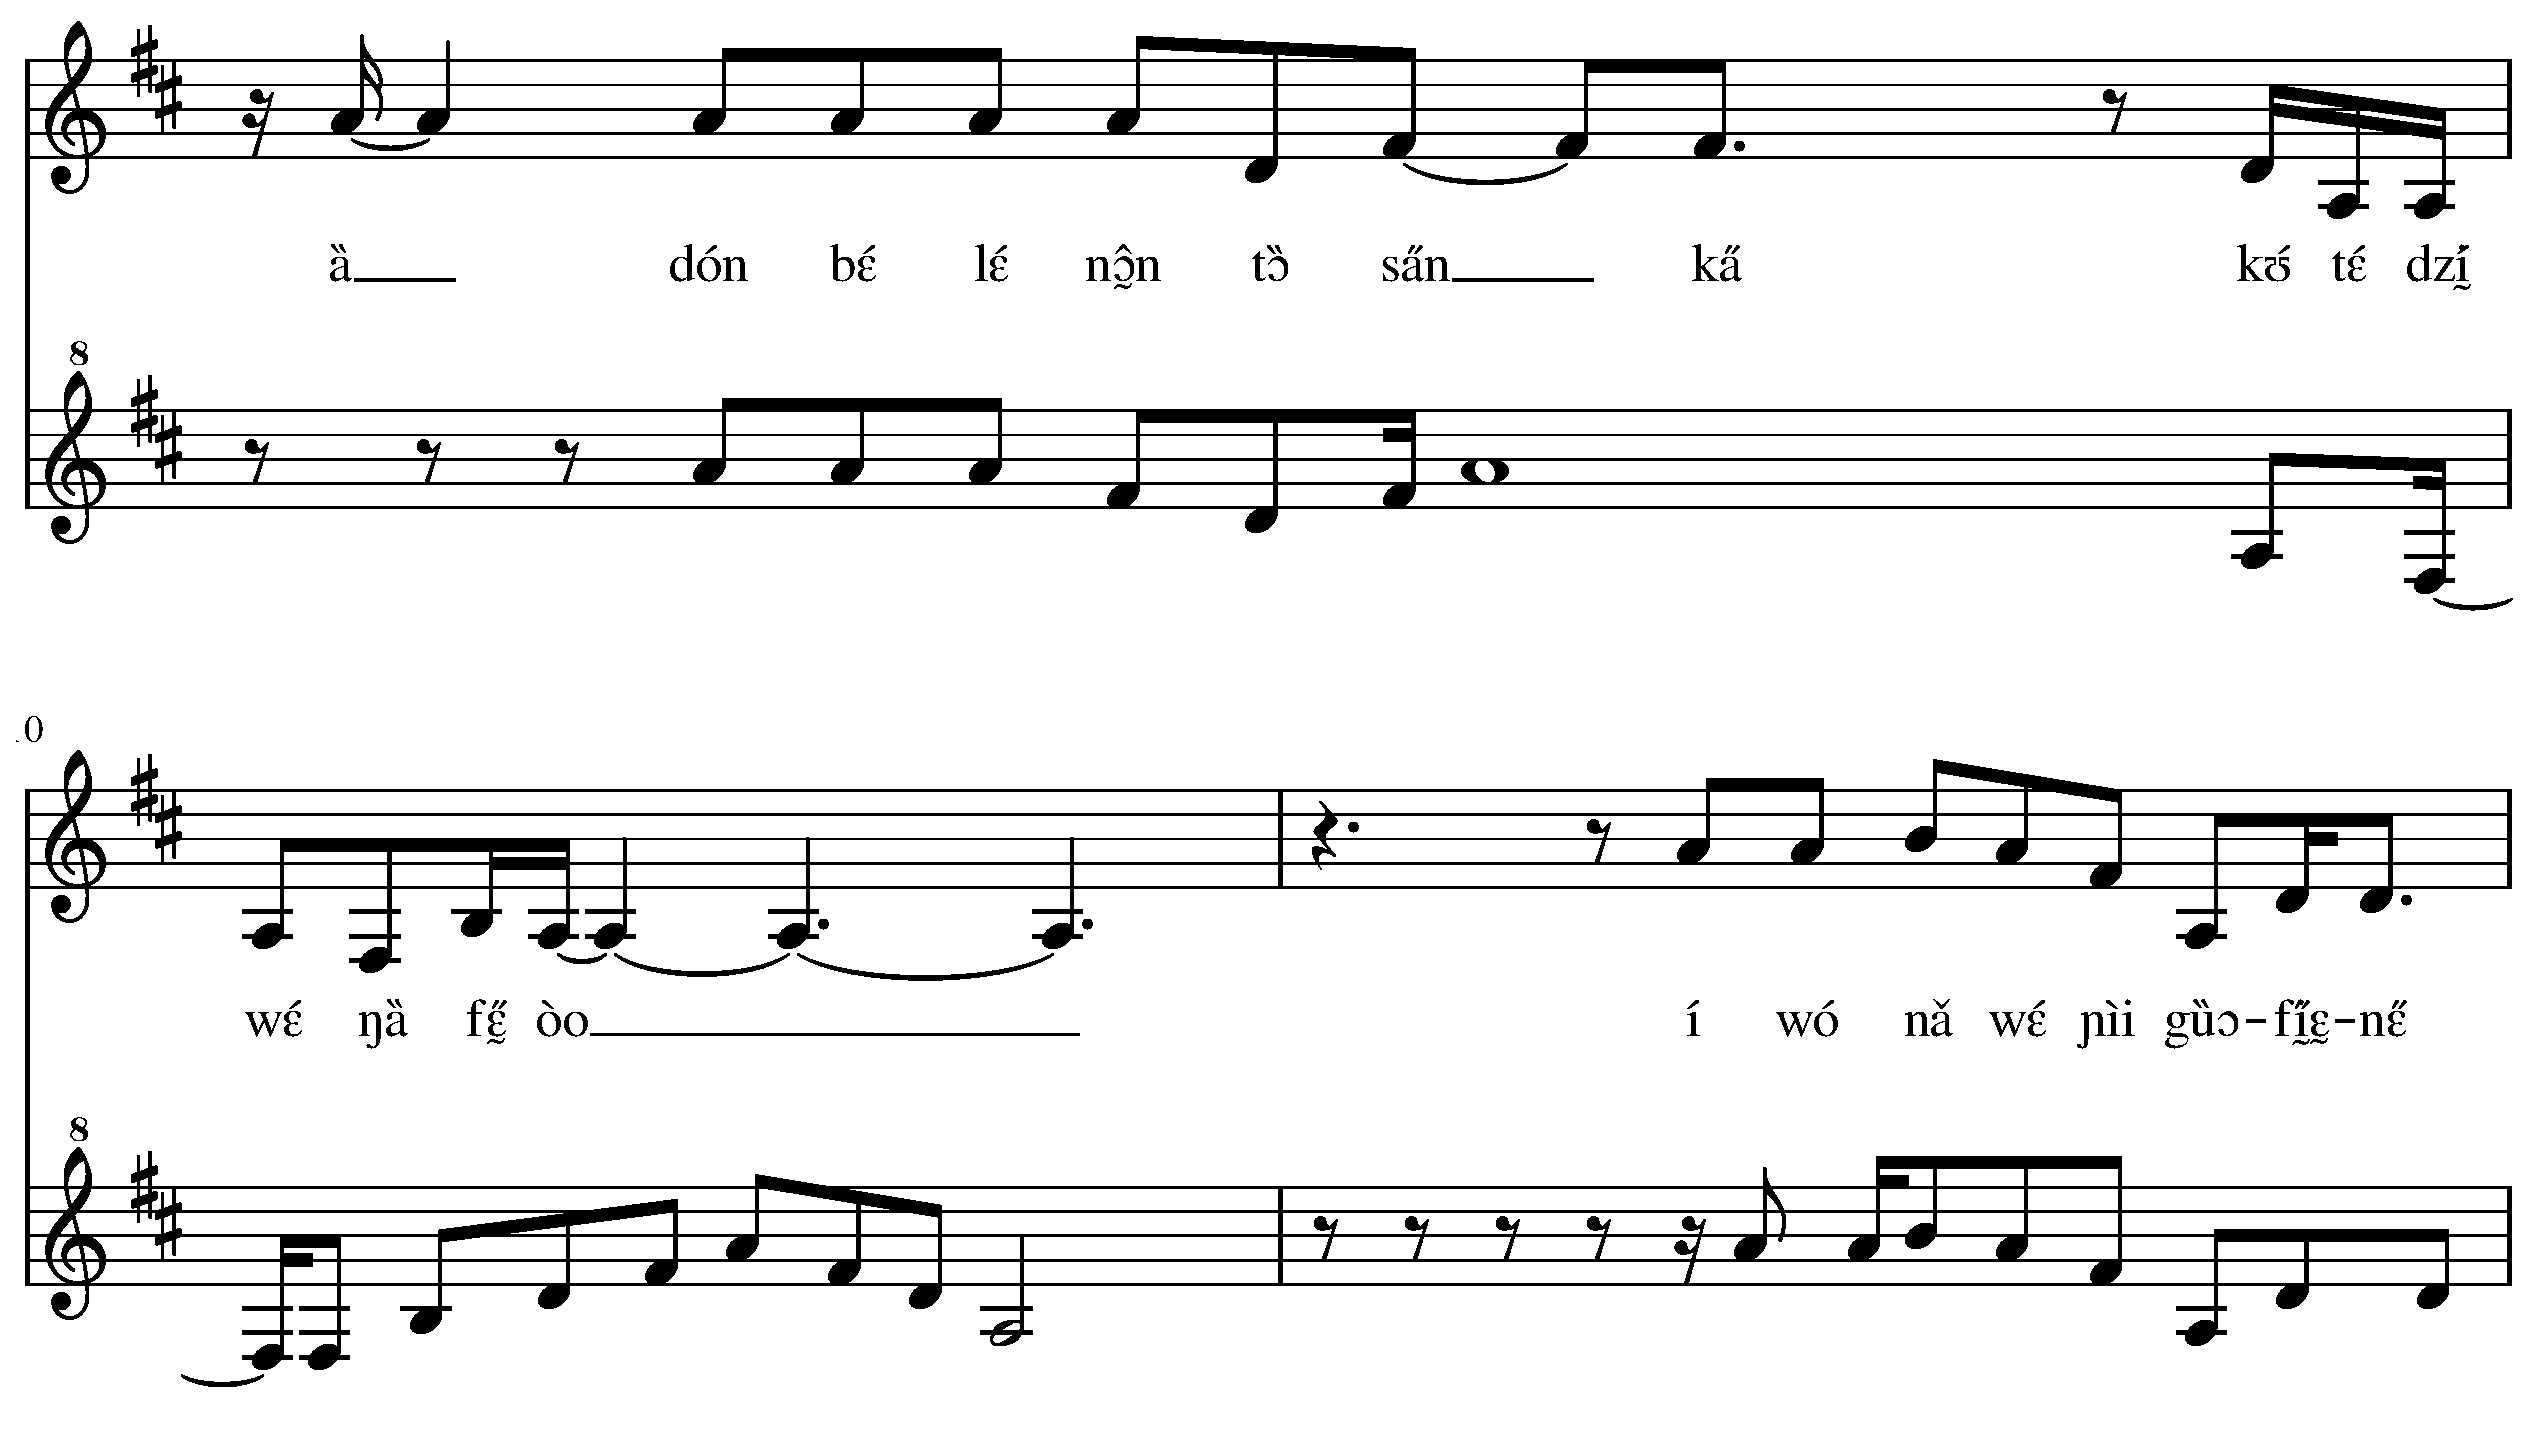
\includegraphics[scale=.37, angle=90]{figures/voice-balafon-comparison.eps}
\caption{Vocal and balafon renditions of lines from \textit{Chief of Bouendé's Song}\label{fig:mcpherson:Bouende}} 
\end{figure}

From these lines, we can see that the vocal rendition and the balafon rendition are not entirely the same. In some places, for instance, such as when the singer sings \textit{fɛ̰̋ òo}, the balafon launches into a more musical flourish. In other places, the melody is almost exactly the same. Musicians have told us that in many cases, lyrics like these are learned as music first and thus are not tightly tied to language. However, this must not universally be the case, since an interesting point stands out in \figref{fig:mcpherson:Bouende}: While the vocal line encodes postlexical tone through rising tone simplification on \textit{nǎ} (bottom stave), this simplification is ``undone'' in the balafon rendition, placing the balafon's version one step closer to the deep level of encoding seen in regular surrogate speech. 

There may well be differences between musicians in how linguistic their surrogate singing is. The example we have provided here was played in 1985 by the master balafonist Penegue Diabate, who was the head of balafon clan at the time. It may be that younger musicians or those less familiar with the vocal tradition may not actively think of the words in the same way, leading to greater deviations from expected linguistic encoding. More in-depth investigation of this point will need to await future research. 


\section{Discussion}\label{sec-discussion}

The main findings of this paper are summarized in \tabref{tab:mcpherson:Mainfindings}.

\begin{table}
\caption{Main findings for musical adaptation of tone\label{tab:mcpherson:Mainfindings}}
\fittable{\begin{tabular}{llll} 
\lsptoprule
& {Surrogate speech} & {Surrogate singing} & {Vocal music} \\ \midrule
{Tone-note correspondence}   & Absolute(-ish) & Relative & Relative \\ 
{Contour tones} & Encoded & Variable & Simplified \\ 
{Grammatical tone} & Encoded & Encoded & Encoded \\
{Postlexical tone} & Not encoded & Variable & Encoded \\ 
\lspbottomrule
\end{tabular}}
\end{table}

Thus, we have seen that musical adaptation of tone is not monolithic. We find differences in the level of encoding across musical modalities for even a single language like Seenku, with surrogate speech showing a tighter match between tone and note than vocal music and also a deeper level of encoding; surrogate singing falls somewhere in between. At the same time, we also find similarities in encoding across languages for a single modality, with Seenku tonal textsetting closely resembling what has been reported for other vocal traditions in Africa and beyond. 

Returning to the question of level of encoding, we find that vocal music is encoded at a much more surface level than surrogate speech, which encodes lexical and grammatical tone (what could be perceived as the output of the morphological component) but no phonological or postlexical rules. Here we speculate on some possible reasons for these differences. First, there is a different function for surrogate speech vs. vocal music; the latter is a form of pure artistic expression, meant to be aesthetically pleasing, while surrogate speech is first and foremost a means of communication. This may allow artistic freedom in how tones are set to melodies in vocal music that are not afforded to surrogate speech, which must relay a message. Going further on this point, we also find different structural constraints between the two systems in terms of communicating a linguistic message. Vocal music benefits from having the full range of segmental contrasts available as the person sings, whereas in surrogate speech, the language is stripped back to simply tone and rhythm. It may be, then, that encoding something closer to the underlying form helps the listening recover the message, especially if postlexical processes are neutralizing, as is the case in Seenku. Finally, the two modalities differ in their physiology. Vocal music uses the same apparatus as speech (the vocal tract), which certainly brings it closer to regular speech production, while the linguistic content is displaced to the hands in surrogate speech. 

More work must be done to begin to disentangle these effects and determine how widespread this pattern of difference is cross-linguistically. While the literature contains a good number of studies of tonal textsetting, we could still use more, especially studies that actively report on precisely which kinds of tone serve as the input (lexical, grammatical, postlexical, etc.). We are still sorely lacking in phonologically-oriented studies of musical surrogate speech, leaving only very few points of comparison with the Seenku results. Many more studies are needed to begin to identify common trends or universals in this modality. Finally, we also need more studies comparing multiple modalities within a single language, e.g. tonal adaptation in Yorùbá vocal music vs. drummed speech. These are areas ripe for discovery that stand to shed light on what it is that humans do when adapting their phonological structure to musical form. 

\section*{Abbreviations}

Below are listed only those abbreviations that do not adhere to or are beyond the scope of the Leipzig Glossing Rules.

\begin{multicols}{3}
\begin{tabbing}
   \textsc{prosp}\hspace{1em}\= prospective\kill
   \textsc{emph} \> emphatic\\
   \textsc{excl} \> exclamative\\
   \textsc{nom} \> nominal\\
   \textsc{prosp} \> prospective\\
   \textsc{red} \> reduplicant\\
\end{tabbing}
\end{multicols}

\section*{Acknowledgments}

We would like to thank the audiences at ACAL 50, U Mass, UCSC, and NYU, as well as two anonymous reviewers, for helpful feedback on this work. We are indebted to the Sambla musicians and consultants who shared their music and language with us, especially Mamadou Diabate, Sadama Diabate, Nigo Diabate, Yacouba Konate, Emma Traore, Clement Traore, Fatou Traore, Ga Kənɔn Traore, Ga Masa Traore, Go Gardi Traore, and Sadiouma Traore. This material is based upon work supported by the National Science Foundation-National Endowment for the Humanities Documenting Endangered Languages Program under National Science Foundation Award No. BCS-1664335 and by funding from the Dartmouth College Leslie Center for the Humanities. 


{\sloppy\printbibliography[heading=subbibliography,notkeyword=this]}
\end{document}
